Anacleta, ciclista apasionada,
está en la ciudad A planificando su recorrido para los próximos días.
En su mapa, nota que desde allí puede pedalear hacia las ciudades B y C,
que están a 16 y 21 kilómetros de distancia, respectivamente:

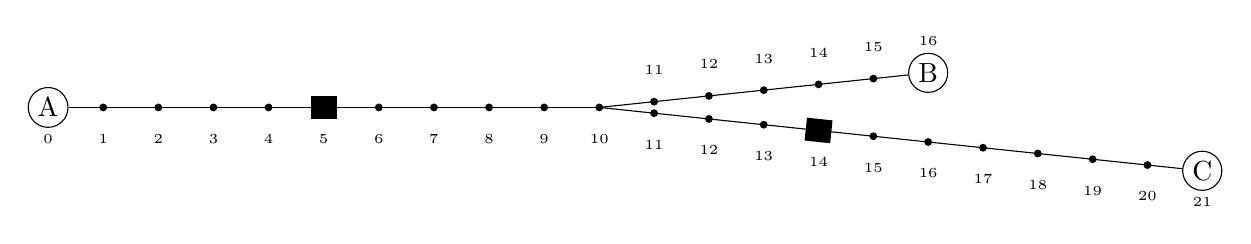
\begin{tikzpicture}[scale=.7]
  \def\forkangle{6}
  \node[draw, circle, inner sep=1.5pt] (A) at (180:10cm)         {A};
  \node[draw, circle, inner sep=1.5pt] (B) at (+\forkangle:6cm)  {B};
  \node[draw, circle, inner sep=1.5pt] (C) at (-\forkangle:11cm) {C};
  \coordinate (Y) at (0, 0);
  \coordinate (p1) at (180:5cm);
  \coordinate (p2) at (-\forkangle:4cm);
  \draw (A) -- (Y);
  \draw (Y) -- (B);
  \draw (Y) -- (C);
  \node[fill, inner sep=2pt] at (p1) {x};
  \node[fill, inner sep=2pt, rotate=-\forkangle] at (p2) {x};
  \foreach\i in {0,...,9} {
    \edef\dist{\i\noexpand cm}
    \node[circle, fill, inner sep=1pt] (x) at (180:\dist) {};
    %\node[yshift=-1cm, anchor=north] (l) at (180:\dist) {{10 - \i}};
  }
  \foreach\i in {1,...,5} {
    \edef\dist{\i\noexpand cm}
    \node[circle, fill, inner sep=1pt] (x) at (+\forkangle:\dist) {};
    %\node[yshift=-1cm, anchor=north] (l) at (180:\dist) {{10 - \i}};
  }
  \foreach\i in {1,...,10} {
    \edef\dist{\i\noexpand cm}
    \node[circle, fill, inner sep=1pt] (x) at (-\forkangle:\dist) {};
    %\node[yshift=-1cm, anchor=north] (l) at (180:\dist) {{10 - \i}};
  }

  \def\labeldist{.4cm}
  \tikzstyle{kmlabel}=[font=\tiny]
  \foreach\km in {0,...,10} {
    \node[yshift=-\labeldist, kmlabel] at (180:{10 - \km}) {\km};
  }
  \foreach\km in {11,...,21} {
    \node[yshift=-\labeldist, kmlabel] at (-\forkangle:{\km - 10}) {\km};
  }
  \foreach\km in {11,...,16} {
    \node[yshift=+\labeldist, kmlabel] at (+\forkangle:{\km - 10}) {\km};
  }
\end{tikzpicture}

Anacleta sólo puede pedalear una cantidad limitada de kilómetros en un día
(que denominaremos su \emph{autonomía}),
por lo que decide avanzar cada día lo más que pueda,
y acampar junto al camino por la noche.

Sin embargo,
hay lugares en el camino (marcados en el mapa con un cuadrado negro)
que son extremadamente peligrosos.
Anacleta es una mujer sensata:
decide evitar acampar en esos puntos,
y planifica hacerlo un kilómetro antes
cuando sea necesario para evitar los peligros.

Escriba un programa que reciba como entradas
el destino y la autonomía de Anacleta,
y le indique en qué puntos del camino
debe acampar cada noche.

\begin{minipage}[t]{.26\textwidth}
  \lstinputlisting[language=testcase,frame=single,linerange=CASO\ 1-FIN\ CASO\ 1]{anacleta/casos.txt}
\end{minipage}
\hfil
\begin{minipage}[t]{.26\textwidth}
  \lstinputlisting[language=testcase,frame=single,linerange=CASO\ 2-FIN\ CASO\ 2]{anacleta/casos.txt}
\end{minipage}
\hfil
\begin{minipage}[t]{.26\textwidth}
  \lstinputlisting[language=testcase,frame=single,linerange=CASO\ 3-FIN\ CASO\ 3]{anacleta/casos.txt}
\end{minipage}

